\documentclass{mooiman_memo}
\addbibresource{./ref.bib}

\newcommand{\ii}{{\rm i}}
\newcommand{\Dx}{\Delta x}
\newcommand{\Dy}{\Delta y}
\newcommand{\Dt}{\Delta t}
\renewcommand{\vec}[1]{\mbox{\boldmath $#1$} }
\newcommand{\mat}[1]{\mbox{\boldmath ${\rm #1}$} }
\newcommand{\half}{\frac{1}{2}}
\newcommand{\quart}{\frac{1}{4}}
\newcommand{\abs}[1]{\left| #1 \right|}
\newcommand{\Sabs}{\textsl{Sabs}\xspace}
\newcommand{\eps}{\varepsilon}

\newcommand{\rhsadv}{{\it rhs}_{\it adv}}
\newcommand{\rhsmom}{{\it rhs}_{\it mom}}
\newcommand{\rhscont}{{\it rhs}_{\it cont}}
\newcommand{\GRADc}{{\it \widehat{GRAD}}_{\it c}}
\newcommand{\GRADu}{{\it \widehat{GRAD}}_{\it u}}
\newcommand{\GRADh}{{\it \widehat{GRAD}}_{\it h}}

\newcommand{\deltares}{Deltares\xspace}
\newcommand{\smartnumerics}{SMART numerics\xspace}
\newcommand{\maplemath}{\textbf{Some MapleSoft math}}

\begin{document}
    \memoTo{???}
    \memoConfidentialUntil{}
    \memoDate{\today~\currenttime}
    \memoVersion{001}
    \memoFrom{Jan Mooiman}
    \memoTelephone{+31\,(0)6\,4691\,4571}
    \memoEmail{jan.mooiman@deltares.nl}
    \memoSubject{Brusselator}
    \memoCopy{}

    \mooimantitle
    %------------------------------------------------------------------------------

\section{Brusselator}
The Brusselator is taken as example to see the behaviour or the fully implicit $\Delta$-formulation for reaction terms only.
This particularly of interest for the water quality computations with lots of processes.
Example taken from \citet{AultHolmgreen2003}.

The  ODE system reads:
\begin{align}
    \pdiff{u_1}{t} & = 1 - (k_2 + 1) u_1 + k_1 u_1^2 u_2,
    \\
    \pdiff{u_2}{t} & = k_2 u_1 - k_1 u_1^2 u_2
\end{align}
with $k_1 =1$ and  $k_2 = 2.5$ and initial values  $u_1(0)=0$ and $u_2(0) = 0$.
%The exact solution reads:
%\begin{align}
%w_1(t) & =\frac{k_2}{k_1+k_2}\left( w_1(0) + w_2(0) \right)
%+ \frac{\exp\left( -(k_1 + k_2)t \right)}{k_1+k_2}\left(   k_1 w_1(0) - k_2 w_2(0) \right),
%\\
%w_2(t) & = \frac{k_2}{k_1+k_2}\left( w_1(0) + w_2(0) \right)
%- \frac{\exp\left( -(k_1 + k_2)t \right)}{k_1+k_2}\left(   k_1 w_1(0) - k_2 w_2(0) \right).
%\end{align}
%after a short time the term $\exp\left( -(k_1 + k_2)t \right)$ is negligible.
%
%
%
Some results are:
\begin{figure}[H]
    \begin{subfigure}{\textwidth}
        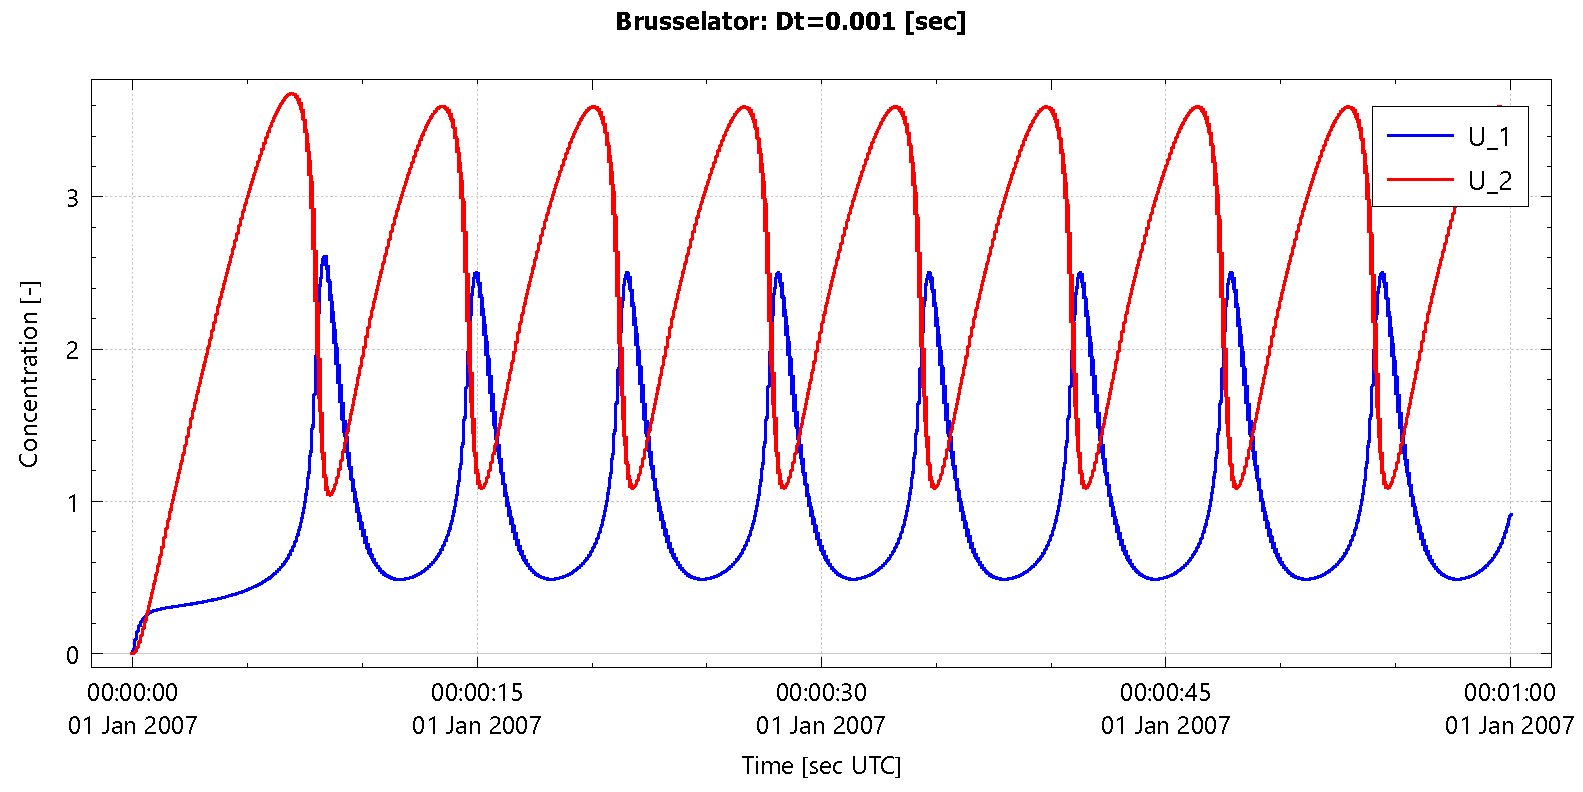
\includegraphics[width=\textwidth]{figures/brusselator_rk4_dt=0d001.pdf}
        \caption{Runge-Kutta 4: $\Dt=0.001$, $k_1=1$, $k_2=2.5$}
    \end{subfigure}
\end{figure}
\begin{figure}[H]\ContinuedFloat
        \begin{subfigure}{0.5\textwidth}
        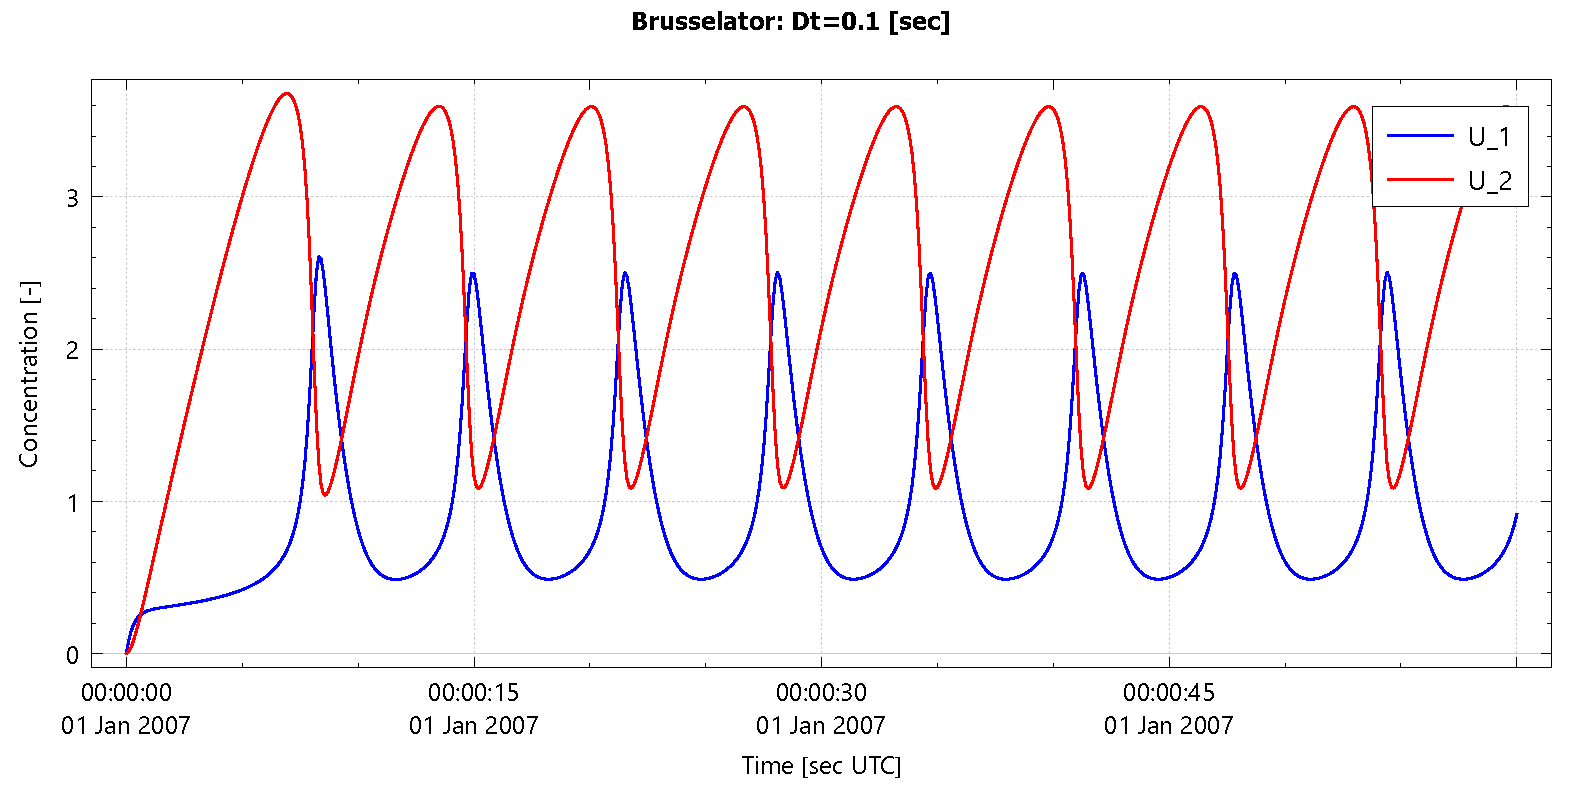
\includegraphics[width=\textwidth]{figures/brusselator_rk4_dt=0d10.pdf}
        \caption{Runge-Kutta 4: $\Dt=0.1$, $k_1=1$, $k_2=2.5$}
    \end{subfigure}
    \begin{subfigure}{0.5\textwidth}
        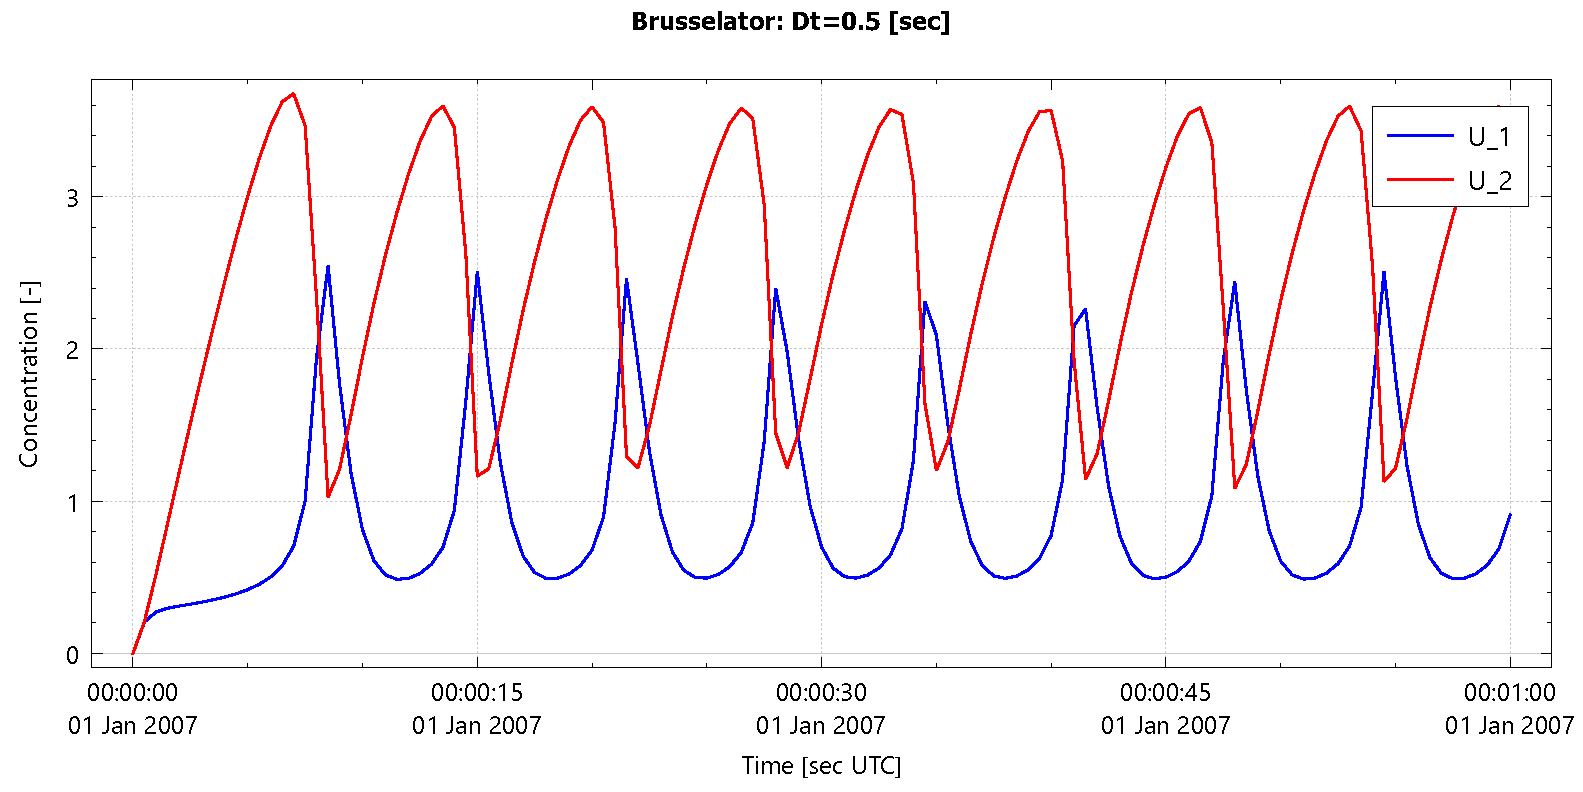
\includegraphics[width=\textwidth]{figures/brusselator_rk4_dt=0d50.pdf}
        \caption{Runge-Kutta 4: $\Dt=0.5$, $k_1=1$, $k_2=2.5$}
    \end{subfigure}
\end{figure}
\begin{figure}[H]\ContinuedFloat
    \begin{subfigure}{0.49\textwidth}
    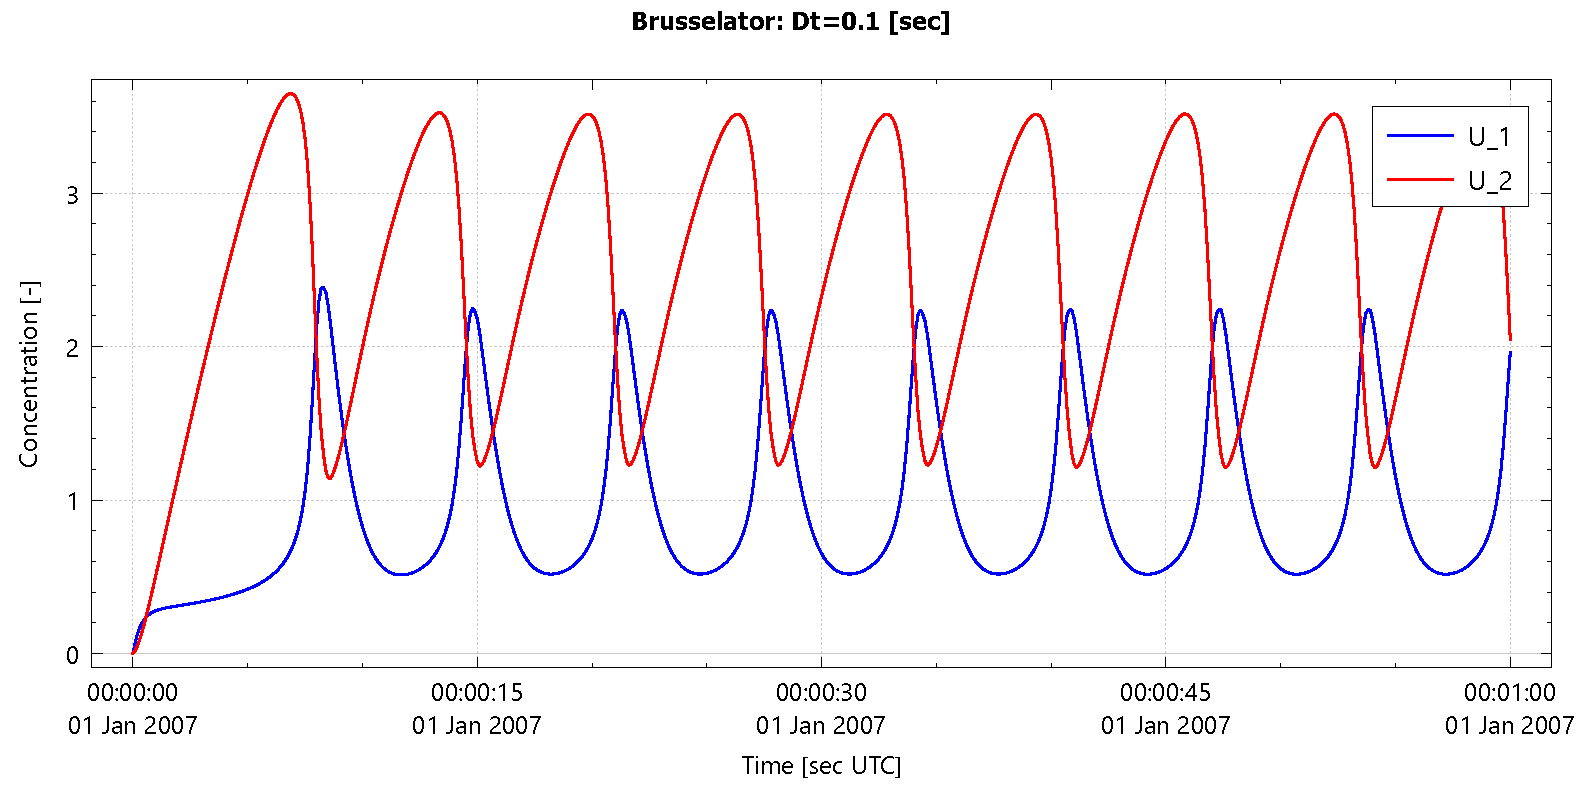
\includegraphics[width=\textwidth]{figures/brusselator_imp_dt=0d10.pdf}
    \caption{Fully Implicit: $\Dt=0.1$, $k_1=1$, $k_2=2.5$}
    \end{subfigure}
    \hfill
    \begin{subfigure}{0.49\textwidth}
        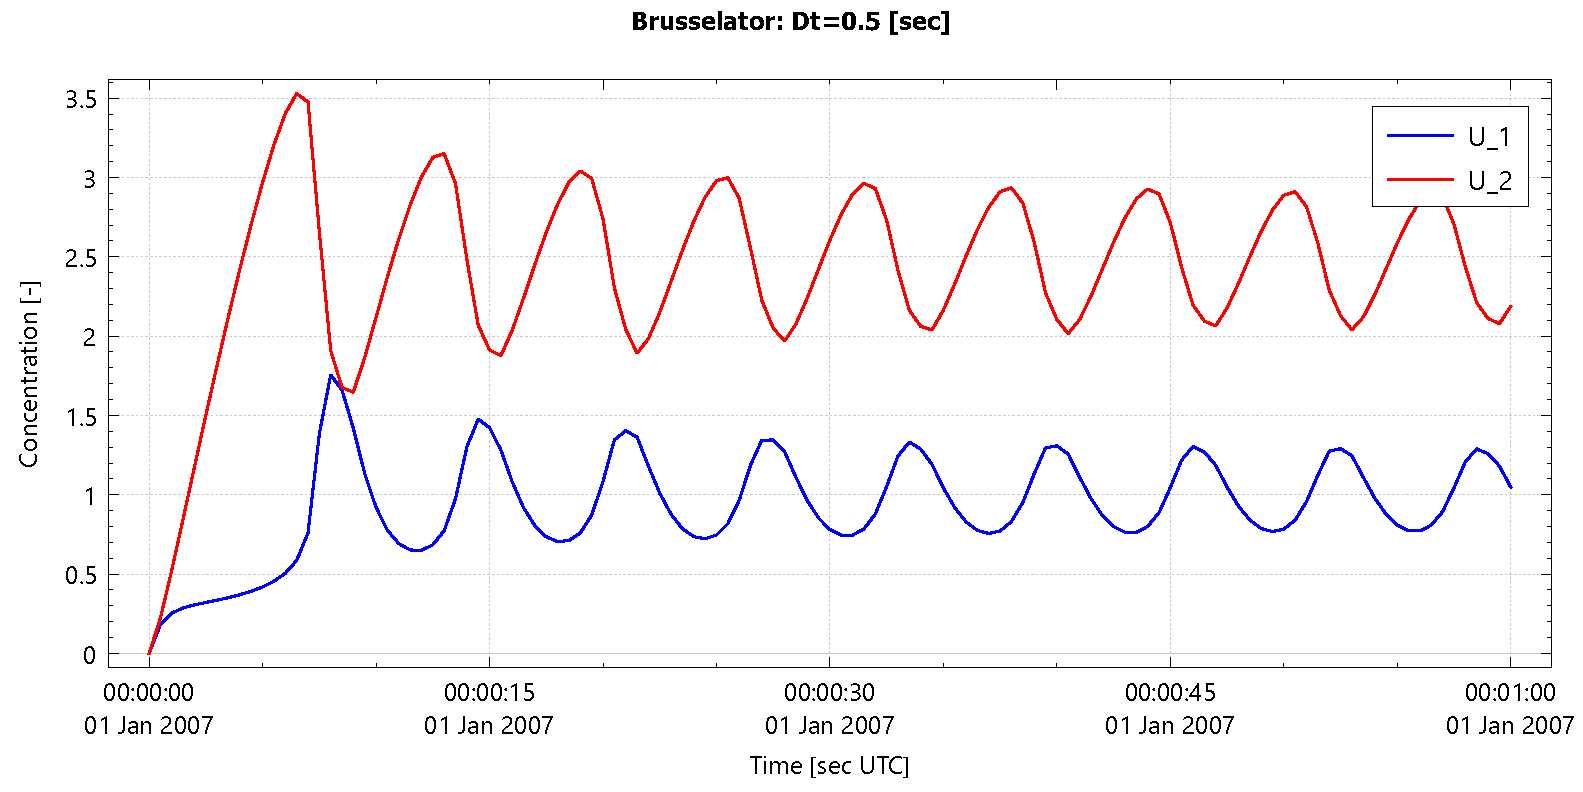
\includegraphics[width=\textwidth]{figures/brusselator_imp_dt=0d50.pdf}
        \caption{Fully Implicit: $\Dt=0.5$, $k_1=1$, $k_2=2.5$}
    \end{subfigure}
    \caption{Result plots for constant value of $k_1 = 1$ and $k_2 =2.5$, computed with a Runge-Kutta 4 and fully implicit ($\Delta$-formulation) time integration method for different time steps $\Dt = 0.1, 0.5$.
    }
\end{figure}
Extra attention needed for the Fully Implicit time integration with larger time step:
\begin{figure}[H]
    \begin{subfigure}{0.49\textwidth}
        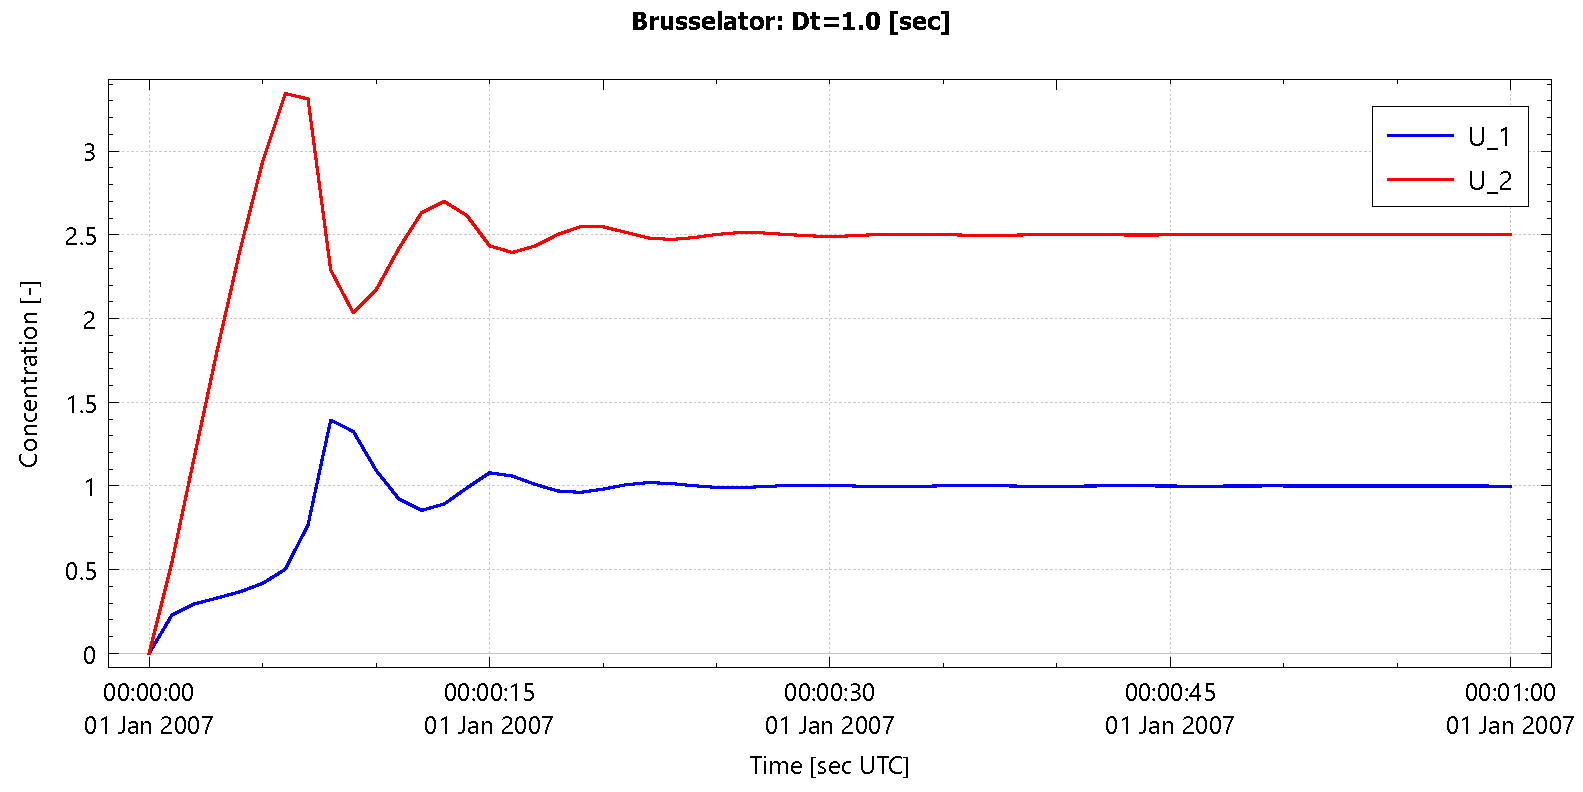
\includegraphics[width=\textwidth]{figures/brusselator_imp_dt=1d00.pdf}
        \caption{Fully Implicit: $\Dt=1.0$, $k_1=1$, $k_2=2.5$}\label{fig:imp_dt=1d00}
    \end{subfigure}
    \hfill
    \begin{subfigure}{0.49\textwidth}
        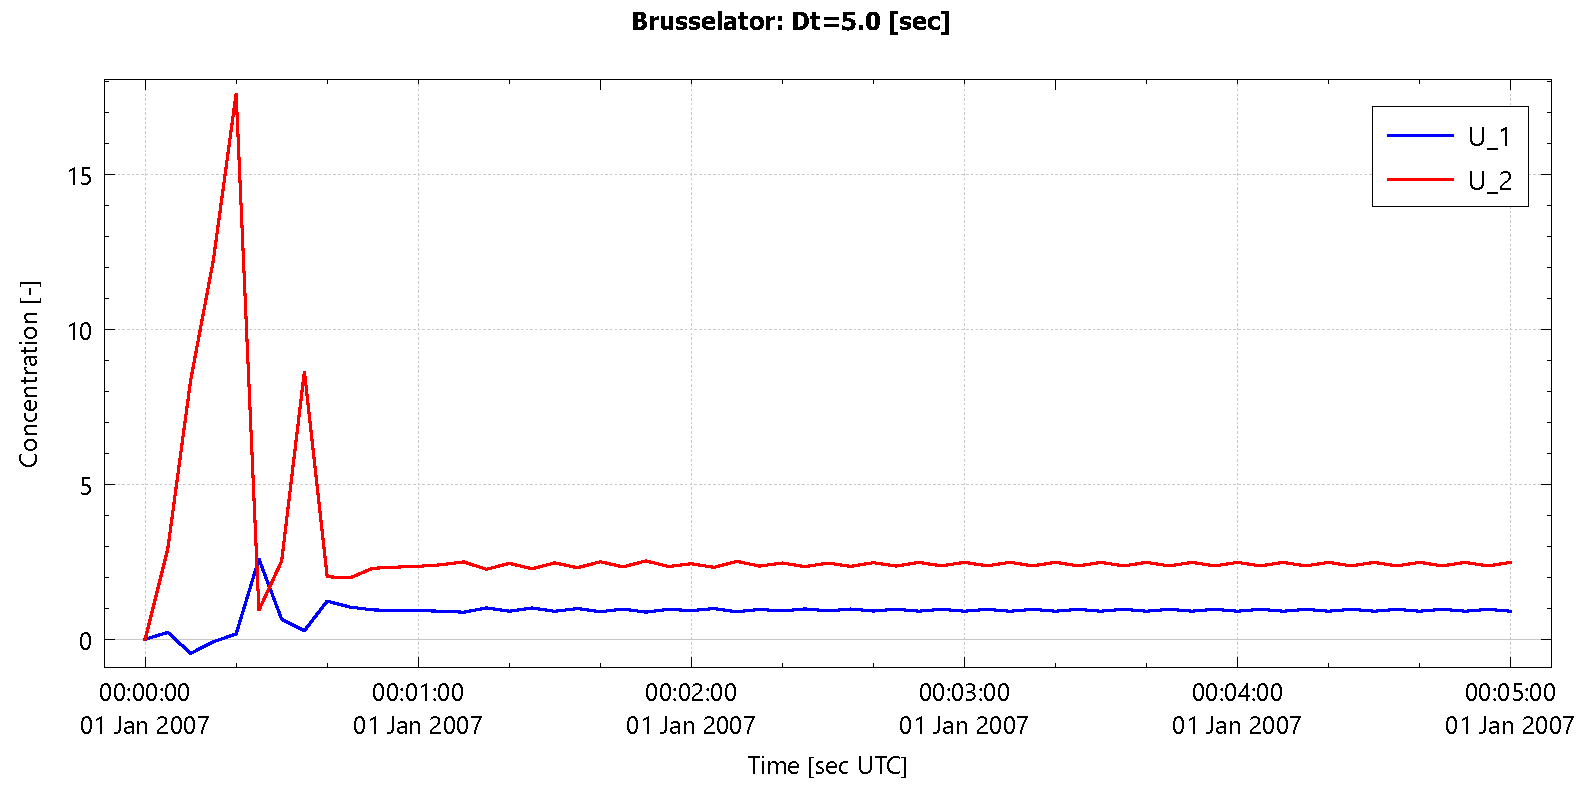
\includegraphics[width=\textwidth]{figures/brusselator_imp_dt=5d00.pdf}
        \caption{Fully Implicit: $\Dt=5.0$, $k_1=1$, $k_2=2.5$}\label{fig:imp_dt=5d00}
    \end{subfigure}
    \caption{Result plots for constant value of $k_1 = 1$ and $k_2 =2.5$, computed with a fully implicit ($\Delta$-formulation) time integration method for different time steps $\Dt = 1.0, 5.0$.
    }
\end{figure}
\Autoref{fig:imp_dt=1d00} converge to the equilibrium state $(u_1, u_2) = (1.0, 2.5)$ and
\Autoref{fig:imp_dt=5d00} looks to converge to the equilibrium state $(u_1, u_2) = (1.0, 2.5)$ but is still wiggling after \SI{5}{\minute} of simulation time (even after one day --- not presented).
%
%%-------------------------------------------------------------------------------
%\section{Numerics}
%Discretized
%\begin{align}
%    \frac{1}{\Dt}\Delta u_1^{n+1, p+1} & = - \frac{1}{\Dt}(u_1^{n+1,p} - u_1^n) - k_1 (u_1^{n+\theta,p+1}) + k_2 (u_2^{n+\theta,p+1})
%    \\
%    \frac{1}{\Dt}\Delta u_2^{n+1, p+1} & = - \frac{1}{\Dt}(u_2^{n+1,p} - u_2^n) + k_1(u_1^{n+\theta,p+1}) - k_2 (u_2^{n+\theta,p+1})
%\end{align}
%Linearization of $\vec{u}^{n+\theta,p+1}$:
%\begin{align}
%    \frac{1}{\Dt}\Delta u_1^{n+1, p+1} & =
%    - \frac{1}{\Dt}(u_1^{n+1,p} - u_1^n) + \\
%    & - k_1 (u_1^{n+\theta,p} + \theta \Delta u_1^{n+1, p+1})
%      + k_2 (u_2^{n+\theta,p} + \theta \Delta u_2^{n+1, p+1})
%    \\
%    \frac{1}{\Dt}\Delta u_2^{n+1, p+1} & = - \frac{1}{\Dt}(u_2^{n+1,p} - u_2^n) +
%    \\
%    & + k_1 (u_1^{n+\theta,p} + \theta \Delta u_1^{n+1, p+1})
%      - k_2 (u_2^{n+\theta,p} + \theta \Delta u_2^{n+1, p+1})
%\end{align}
%Rearrange to $\mat{A}\vec{x}=\vec{b}$
%\begin{align}
%    \frac{1}{\Dt}\Delta u_1^{n+1, p+1} & + k_1 \theta \Delta u_1^{n+1, p+1} - k_2 \theta \Delta u_2^{n+1, p+1} =
%    \\
%& = - \frac{1}{\Dt}(u_1^{n+1,p} - u_1^n) - k_1 u_1^{n+\theta,p} + k_2 u_2^{n+\theta,p}
%\\
%\frac{1}{\Dt}\Delta u_2^{n+1, p+1} & - k_1 \theta \Delta u_1^{n+1, p+1} + k_2 \theta \Delta u_2^{n+1, p+1} = \\
%& =- \frac{1}{\Dt}(u_2^{n+1,p} - u_2^n) + k_1 u_1^{n+\theta,p}
%- k_2 u_2^{n+\theta,p}
%\end{align}
%
%
%%------------------------------------------------------------------------------
\section{Numerical experiment}
%
%--- begin light blue table ---
\begin{longtable}{>{\bfseries}p{6mm-12pt}|p{\textwidth/3-2mm-12pt}|p{\textwidth/3-2mm-12pt}|p{\textwidth/3-2mm-12pt}}
\caption{Stability of different time integrators for the Brusselator.}\\%
\rowcolor{kobaltblue}
& {\textcolor{white}{\textbf{Time step\newline [s]}}}
& {\textcolor{white}{\textbf{Runge-Kutta 4}}}
& {\textcolor{white}{\textbf{Fully Implicit\newline $\Delta$-formulation}}}
\\
\topline
\endfirsthead
\rowcolor{kobaltblue}
& {\textcolor{white}{\textbf{Time step\newline [s]}}}
& {\textcolor{white}{\textbf{Runge-Kutta 4}}}
& {\textcolor{white}{\textbf{Fully Implicit\newline $\Delta$-formulation}}}
\\
\midline
\endhead
\endfoot
\endlastfoot
1 & 0.1 & \checkmark & \checkmark  \\
\midline
2 & 0.2  & \checkmark &  \checkmark   \\
\midline
3 & 0.5 & \checkmark &  \checkmark   \\
\midline
4 & 1.0 & Unstable &   \checkmark  \\
\midline
5 & 2.0 &   &   \checkmark  \\
\midline
6 & 5.0 &   &   \checkmark \\
\bottomline
\end{longtable}
%--- end light blue table ---
%

%------------------------------------------------------------------------------
\printallbibliography
\end{document}
